\documentclass[12pt]{standalone}

\RequirePackage{times}
\RequirePackage{amsmath}
\RequirePackage{amssymb}
\RequirePackage[T1]{fontenc}

\usepackage{tikz}
\usepackage{xcolor}
\usepackage{pgfplots}
\pgfplotsset{compat=1.16}
\usetikzlibrary{arrows}
\pgfdeclarelayer{foreground}
\pgfsetlayers{main,foreground}

\begin{document}
	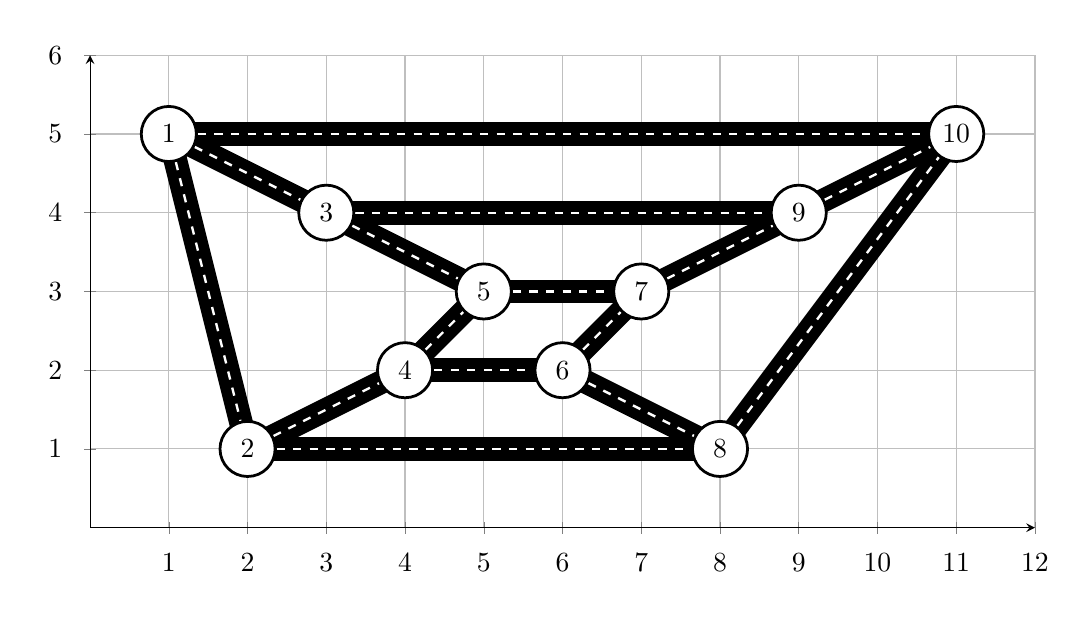
\begin{tikzpicture}[x=1cm,y=1cm,every node/.style={circle,inner sep=0pt,line width=1pt, minimum size = 0.7cm}]
		\begin{axis}[
			x=1.0cm,y=1.0cm,
			axis lines=middle,
			ymajorgrids=true,
			xmajorgrids=true,
			xmin=0,
			xmax=12,
			ymin=0,
			ymax=6,
			xtick={0.0,...,12.0},
			ytick={0.0,...,6.0},]	
			\begin{pgfonlayer}{foreground}
				\node[draw,fill=white] at (1cm,5cm) (v1) {1};
				\node[draw,fill=white] at (2cm,1cm) (v2) {2};
				\node[draw,fill=white] at (3cm,4cm) (v3) {3};
				\node[draw,fill=white] at (4cm,2cm) (v4) {4};
				\node[draw,fill=white] at (5cm,3cm) (v5) {5};
				\node[draw,fill=white] at (6cm,2cm) (v6) {6};
				\node[draw,fill=white] at (7cm,3cm) (v7) {7};
				\node[draw,fill=white] at (8cm,1cm) (v8) {8};
				\node[draw,fill=white] at (9cm,4cm) (v9) {9};
				\node[draw,fill=white] at (11cm,5cm) (v10) {10};
			\end{pgfonlayer}
			\draw[-,line width=0.3cm] (v1.center) -- (v2.center);
			\draw[-,line width=0.3cm] (v1.center) -- (v3.center);
			\draw[-,line width=0.3cm] (v1.center) -- (v10.center);
			\draw[-,line width=0.3cm] (v2.center) -- (v4.center);
			\draw[-,line width=0.3cm] (v3.center) -- (v5.center);
			\draw[-,line width=0.3cm] (v4.center) -- (v5.center);
			\draw[-,line width=0.3cm] (v4.center) -- (v6.center);
			\draw[-,line width=0.3cm] (v5.center) -- (v7.center);
			\draw[-,line width=0.3cm] (v6.center) -- (v7.center);
			\draw[-,line width=0.3cm] (v6.center) -- (v8.center);
			\draw[-,line width=0.3cm] (v7.center) -- (v9.center);
			\draw[-,line width=0.3cm] (v8.center) -- (v10.center);
			\draw[-,line width=0.3cm] (v9.center) -- (v10.center);
			\draw[-,line width=0.3cm] (v2.center) -- (v8.center);
			\draw[-,line width=0.3cm] (v3.center) -- (v9.center);
			
			\draw[dashed,white,line width=0.03cm] (v1) -- (v2);
			\draw[dashed,white,line width=0.03cm] (v1) -- (v3);
			\draw[dashed,white,line width=0.03cm] (v1) -- (v10);
			\draw[dashed,white,line width=0.03cm] (v2) -- (v4);
			\draw[dashed,white,line width=0.03cm] (v3) -- (v5);
			\draw[dashed,white,line width=0.03cm] (v4) -- (v5);
			\draw[dashed,white,line width=0.03cm] (v4) -- (v6);
			\draw[dashed,white,line width=0.03cm] (v5) -- (v7);
			\draw[dashed,white,line width=0.03cm] (v6) -- (v7);
			\draw[dashed,white,line width=0.03cm] (v6) -- (v8);
			\draw[dashed,white,line width=0.03cm] (v7) -- (v9);
			\draw[dashed,white,line width=0.03cm] (v8) -- (v10);
			\draw[dashed,white,line width=0.03cm] (v9) -- (v10);
			\draw[dashed,white,line width=0.03cm] (v2) -- (v8);
			\draw[dashed,white,line width=0.03cm] (v3) -- (v9);
		\end{axis}
	\end{tikzpicture}
\end{document}